\documentclass[twoside]{book}

% Packages required by doxygen
\usepackage{fixltx2e}
\usepackage{calc}
\usepackage{doxygen}
\usepackage[export]{adjustbox} % also loads graphicx
\usepackage{graphicx}
\usepackage[utf8]{inputenc}
\usepackage{makeidx}
\usepackage{multicol}
\usepackage{multirow}
\PassOptionsToPackage{warn}{textcomp}
\usepackage{textcomp}
\usepackage[nointegrals]{wasysym}
\usepackage[table]{xcolor}

% Font selection
\usepackage[T1]{fontenc}
\usepackage[scaled=.90]{helvet}
\usepackage{courier}
\usepackage{amssymb}
\usepackage{sectsty}
\renewcommand{\familydefault}{\sfdefault}
\allsectionsfont{%
  \fontseries{bc}\selectfont%
  \color{darkgray}%
}
\renewcommand{\DoxyLabelFont}{%
  \fontseries{bc}\selectfont%
  \color{darkgray}%
}
\newcommand{\+}{\discretionary{\mbox{\scriptsize$\hookleftarrow$}}{}{}}

% Page & text layout
\usepackage{geometry}
\geometry{%
  a4paper,%
  top=2.5cm,%
  bottom=2.5cm,%
  left=2.5cm,%
  right=2.5cm%
}
\tolerance=750
\hfuzz=15pt
\hbadness=750
\setlength{\emergencystretch}{15pt}
\setlength{\parindent}{0cm}
\setlength{\parskip}{3ex plus 2ex minus 2ex}
\makeatletter
\renewcommand{\paragraph}{%
  \@startsection{paragraph}{4}{0ex}{-1.0ex}{1.0ex}{%
    \normalfont\normalsize\bfseries\SS@parafont%
  }%
}
\renewcommand{\subparagraph}{%
  \@startsection{subparagraph}{5}{0ex}{-1.0ex}{1.0ex}{%
    \normalfont\normalsize\bfseries\SS@subparafont%
  }%
}
\makeatother

% Headers & footers
\usepackage{fancyhdr}
\pagestyle{fancyplain}
\fancyhead[LE]{\fancyplain{}{\bfseries\thepage}}
\fancyhead[CE]{\fancyplain{}{}}
\fancyhead[RE]{\fancyplain{}{\bfseries\leftmark}}
\fancyhead[LO]{\fancyplain{}{\bfseries\rightmark}}
\fancyhead[CO]{\fancyplain{}{}}
\fancyhead[RO]{\fancyplain{}{\bfseries\thepage}}
\fancyfoot[LE]{\fancyplain{}{}}
\fancyfoot[CE]{\fancyplain{}{}}
\fancyfoot[RE]{\fancyplain{}{\bfseries\scriptsize Generated by Doxygen }}
\fancyfoot[LO]{\fancyplain{}{\bfseries\scriptsize Generated by Doxygen }}
\fancyfoot[CO]{\fancyplain{}{}}
\fancyfoot[RO]{\fancyplain{}{}}
\renewcommand{\footrulewidth}{0.4pt}
\renewcommand{\chaptermark}[1]{%
  \markboth{#1}{}%
}
\renewcommand{\sectionmark}[1]{%
  \markright{\thesection\ #1}%
}

% Indices & bibliography
\usepackage{natbib}
\usepackage[titles]{tocloft}
\setcounter{tocdepth}{3}
\setcounter{secnumdepth}{5}
\makeindex

% Hyperlinks (required, but should be loaded last)
\usepackage{ifpdf}
\ifpdf
  \usepackage[pdftex,pagebackref=true]{hyperref}
\else
  \usepackage[ps2pdf,pagebackref=true]{hyperref}
\fi
\hypersetup{%
  colorlinks=true,%
  linkcolor=blue,%
  citecolor=blue,%
  unicode%
}

% Custom commands
\newcommand{\clearemptydoublepage}{%
  \newpage{\pagestyle{empty}\cleardoublepage}%
}

\usepackage{caption}
\captionsetup{labelsep=space,justification=centering,font={bf},singlelinecheck=off,skip=4pt,position=top}

%===== C O N T E N T S =====

\begin{document}

% Titlepage & ToC
\hypersetup{pageanchor=false,
             bookmarksnumbered=true,
             pdfencoding=unicode
            }
\pagenumbering{alph}
\begin{titlepage}
\vspace*{7cm}
\begin{center}%
{\Large Kyle\textquotesingle{}s Doxygen Test }\\
\vspace*{1cm}
{\large Generated by Doxygen 1.8.13}\\
\end{center}
\end{titlepage}
\clearemptydoublepage
\pagenumbering{roman}
\tableofcontents
\clearemptydoublepage
\pagenumbering{arabic}
\hypersetup{pageanchor=true}

%--- Begin generated contents ---
\chapter{File Index}
\section{File List}
Here is a list of all files with brief descriptions\+:\begin{DoxyCompactList}
\item\contentsline{section}{src/\hyperlink{main_8cpp}{main.\+cpp} }{\pageref{main_8cpp}}{}
\item\contentsline{section}{src/\hyperlink{utility_8cpp}{utility.\+cpp} }{\pageref{utility_8cpp}}{}
\item\contentsline{section}{src/\hyperlink{utility_8hpp}{utility.\+hpp} }{\pageref{utility_8hpp}}{}
\end{DoxyCompactList}

\chapter{File Documentation}
\hypertarget{main_8cpp}{}\section{src/main.cpp File Reference}
\label{main_8cpp}\index{src/main.\+cpp@{src/main.\+cpp}}
{\ttfamily \#include $<$stdio.\+h$>$}\newline
{\ttfamily \#include \char`\"{}utility.\+hpp\char`\"{}}\newline
Include dependency graph for main.\+cpp\+:\nopagebreak
\begin{figure}[H]
\begin{center}
\leavevmode
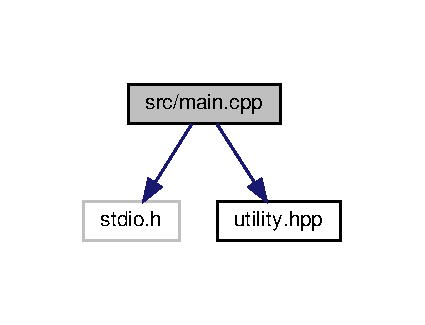
\includegraphics[width=204pt]{main_8cpp__incl}
\end{center}
\end{figure}
\subsection*{Functions}
\begin{DoxyCompactItemize}
\item 
int \hyperlink{main_8cpp_a3c04138a5bfe5d72780bb7e82a18e627}{main} (int argc, char $\ast$$\ast$argv)
\end{DoxyCompactItemize}


\subsection{Function Documentation}
\mbox{\Hypertarget{main_8cpp_a3c04138a5bfe5d72780bb7e82a18e627}\label{main_8cpp_a3c04138a5bfe5d72780bb7e82a18e627}} 
\index{main.\+cpp@{main.\+cpp}!main@{main}}
\index{main@{main}!main.\+cpp@{main.\+cpp}}
\subsubsection{\texorpdfstring{main()}{main()}}
{\footnotesize\ttfamily int main (\begin{DoxyParamCaption}\item[{int}]{argc,  }\item[{char $\ast$$\ast$}]{argv }\end{DoxyParamCaption})}



Definition at line 4 of file main.\+cpp.



References magic(), M\+A\+G\+I\+C\+\_\+\+N\+U\+M\+B\+ER, multiply(), and square().


\begin{DoxyCode}
4                                 \{
5     printf(\textcolor{stringliteral}{"start\(\backslash\)n"});
6     \textcolor{keywordtype}{int} x = 5;
7     \textcolor{keywordtype}{int} y = 6;
8     printf(\textcolor{stringliteral}{"%d squared is %d\(\backslash\)n"}, x, \hyperlink{utility_8cpp_ab12b3cad66448e2bfc8c590d002052da}{square}(x));
9     printf(\textcolor{stringliteral}{"%d times %d is %d\(\backslash\)n"}, x, y, \hyperlink{utility_8cpp_a50de380d6a4786c51a18168d9d9c7fa1}{multiply}(x, y));
10     printf(\textcolor{stringliteral}{"the magic number is %d\(\backslash\)n"}, \hyperlink{utility_8hpp_a54061e5993a5517320d425f44408cc86}{MAGIC\_NUMBER});
11     printf(\textcolor{stringliteral}{"%d magicked is %d\(\backslash\)n"}, x, \hyperlink{utility_8cpp_a07a97f4470961bb441483bc3e8748861}{magic}(x));
12     printf(\textcolor{stringliteral}{"end\(\backslash\)n"});
13     \textcolor{keywordflow}{return} 0;
14 \}
\end{DoxyCode}

\hypertarget{utility_8cpp}{}\section{src/utility.cpp File Reference}
\label{utility_8cpp}\index{src/utility.\+cpp@{src/utility.\+cpp}}
{\ttfamily \#include \char`\"{}utility.\+hpp\char`\"{}}\newline
Include dependency graph for utility.\+cpp\+:\nopagebreak
\begin{figure}[H]
\begin{center}
\leavevmode
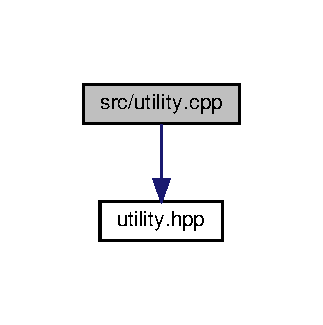
\includegraphics[width=155pt]{utility_8cpp__incl}
\end{center}
\end{figure}
\subsection*{Functions}
\begin{DoxyCompactItemize}
\item 
int \hyperlink{utility_8cpp_ab12b3cad66448e2bfc8c590d002052da}{square} (int x)
\begin{DoxyCompactList}\small\item\em Squares a number. \end{DoxyCompactList}\item 
int \hyperlink{utility_8cpp_a50de380d6a4786c51a18168d9d9c7fa1}{multiply} (int x, int y)
\begin{DoxyCompactList}\small\item\em Multiplies two numbers. \end{DoxyCompactList}\item 
int \hyperlink{utility_8cpp_a07a97f4470961bb441483bc3e8748861}{magic} (int x)
\begin{DoxyCompactList}\small\item\em Function for magic math. \end{DoxyCompactList}\end{DoxyCompactItemize}


\subsection{Function Documentation}
\mbox{\Hypertarget{utility_8cpp_a07a97f4470961bb441483bc3e8748861}\label{utility_8cpp_a07a97f4470961bb441483bc3e8748861}} 
\index{utility.\+cpp@{utility.\+cpp}!magic@{magic}}
\index{magic@{magic}!utility.\+cpp@{utility.\+cpp}}
\subsubsection{\texorpdfstring{magic()}{magic()}}
{\footnotesize\ttfamily int magic (\begin{DoxyParamCaption}\item[{int}]{x }\end{DoxyParamCaption})}



Function for magic math. 

This function multiplies a number by the magic number.


\begin{DoxyParams}{Parameters}
{\em x} & The number on which to perfom magic. \\
\hline
\end{DoxyParams}
\begin{DoxyReturn}{Returns}
The magic product of the number. 
\end{DoxyReturn}


Definition at line 14 of file utility.\+cpp.



References M\+A\+G\+I\+C\+\_\+\+N\+U\+M\+B\+ER.



Referenced by main().


\begin{DoxyCode}
14                  \{
15     \textcolor{keywordflow}{return} \hyperlink{utility_8hpp_a54061e5993a5517320d425f44408cc86}{MAGIC\_NUMBER} * x;
16 \}
\end{DoxyCode}
\mbox{\Hypertarget{utility_8cpp_a50de380d6a4786c51a18168d9d9c7fa1}\label{utility_8cpp_a50de380d6a4786c51a18168d9d9c7fa1}} 
\index{utility.\+cpp@{utility.\+cpp}!multiply@{multiply}}
\index{multiply@{multiply}!utility.\+cpp@{utility.\+cpp}}
\subsubsection{\texorpdfstring{multiply()}{multiply()}}
{\footnotesize\ttfamily int multiply (\begin{DoxyParamCaption}\item[{int}]{x,  }\item[{int}]{y }\end{DoxyParamCaption})}



Multiplies two numbers. 

This function multiplies a number times another number and returns the result of those two numbers multiplied together. The result is the product of the two numbers, and that is the value that is returned by this function.


\begin{DoxyParams}{Parameters}
{\em x} & The first operand. \\
\hline
{\em y} & The second operand. \\
\hline
\end{DoxyParams}
\begin{DoxyReturn}{Returns}
The product. 
\end{DoxyReturn}


Definition at line 10 of file utility.\+cpp.



Referenced by main().


\begin{DoxyCode}
10                            \{
11     \textcolor{keywordflow}{return} x * y;
12 \}
\end{DoxyCode}
\mbox{\Hypertarget{utility_8cpp_ab12b3cad66448e2bfc8c590d002052da}\label{utility_8cpp_ab12b3cad66448e2bfc8c590d002052da}} 
\index{utility.\+cpp@{utility.\+cpp}!square@{square}}
\index{square@{square}!utility.\+cpp@{utility.\+cpp}}
\subsubsection{\texorpdfstring{square()}{square()}}
{\footnotesize\ttfamily int square (\begin{DoxyParamCaption}\item[{int}]{x }\end{DoxyParamCaption})}



Squares a number. 

he 

Definition at line 6 of file utility.\+cpp.



Referenced by main().


\begin{DoxyCode}
6                   \{
7     \textcolor{keywordflow}{return} x * x;
8 \}
\end{DoxyCode}

\hypertarget{utility_8hpp}{}\section{src/utility.hpp File Reference}
\label{utility_8hpp}\index{src/utility.\+hpp@{src/utility.\+hpp}}
This graph shows which files directly or indirectly include this file\+:\nopagebreak
\begin{figure}[H]
\begin{center}
\leavevmode
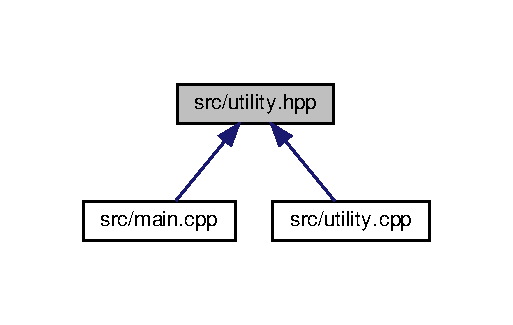
\includegraphics[width=246pt]{utility_8hpp__dep__incl}
\end{center}
\end{figure}
\subsection*{Macros}
\begin{DoxyCompactItemize}
\item 
\#define \hyperlink{utility_8hpp_a54061e5993a5517320d425f44408cc86}{M\+A\+G\+I\+C\+\_\+\+N\+U\+M\+B\+ER}~1337
\begin{DoxyCompactList}\small\item\em Magic number for magical computation. \end{DoxyCompactList}\end{DoxyCompactItemize}
\subsection*{Functions}
\begin{DoxyCompactItemize}
\item 
int \hyperlink{utility_8hpp_ab12b3cad66448e2bfc8c590d002052da}{square} (int x)
\begin{DoxyCompactList}\small\item\em Squares a number. \end{DoxyCompactList}\item 
int \hyperlink{utility_8hpp_a50de380d6a4786c51a18168d9d9c7fa1}{multiply} (int x, int y)
\begin{DoxyCompactList}\small\item\em Multiplies two numbers. \end{DoxyCompactList}\item 
int \hyperlink{utility_8hpp_a07a97f4470961bb441483bc3e8748861}{magic} (int x)
\begin{DoxyCompactList}\small\item\em Function for magic math. \end{DoxyCompactList}\end{DoxyCompactItemize}


\subsection{Macro Definition Documentation}
\mbox{\Hypertarget{utility_8hpp_a54061e5993a5517320d425f44408cc86}\label{utility_8hpp_a54061e5993a5517320d425f44408cc86}} 
\index{utility.\+hpp@{utility.\+hpp}!M\+A\+G\+I\+C\+\_\+\+N\+U\+M\+B\+ER@{M\+A\+G\+I\+C\+\_\+\+N\+U\+M\+B\+ER}}
\index{M\+A\+G\+I\+C\+\_\+\+N\+U\+M\+B\+ER@{M\+A\+G\+I\+C\+\_\+\+N\+U\+M\+B\+ER}!utility.\+hpp@{utility.\+hpp}}
\subsubsection{\texorpdfstring{M\+A\+G\+I\+C\+\_\+\+N\+U\+M\+B\+ER}{MAGIC\_NUMBER}}
{\footnotesize\ttfamily \#define M\+A\+G\+I\+C\+\_\+\+N\+U\+M\+B\+ER~1337}



Magic number for magical computation. 

This number is selected to be the most elite number there is. No other numbers are more elite than this number. 

Definition at line 10 of file utility.\+hpp.



Referenced by magic(), and main().



\subsection{Function Documentation}
\mbox{\Hypertarget{utility_8hpp_a07a97f4470961bb441483bc3e8748861}\label{utility_8hpp_a07a97f4470961bb441483bc3e8748861}} 
\index{utility.\+hpp@{utility.\+hpp}!magic@{magic}}
\index{magic@{magic}!utility.\+hpp@{utility.\+hpp}}
\subsubsection{\texorpdfstring{magic()}{magic()}}
{\footnotesize\ttfamily int magic (\begin{DoxyParamCaption}\item[{int}]{x }\end{DoxyParamCaption})}



Function for magic math. 

This function multiplies a number by the magic number.


\begin{DoxyParams}{Parameters}
{\em x} & The number on which to perfom magic. \\
\hline
\end{DoxyParams}
\begin{DoxyReturn}{Returns}
The magic product of the number. 
\end{DoxyReturn}


Definition at line 14 of file utility.\+cpp.



References M\+A\+G\+I\+C\+\_\+\+N\+U\+M\+B\+ER.



Referenced by main().


\begin{DoxyCode}
14                  \{
15     \textcolor{keywordflow}{return} \hyperlink{utility_8hpp_a54061e5993a5517320d425f44408cc86}{MAGIC\_NUMBER} * x;
16 \}
\end{DoxyCode}
\mbox{\Hypertarget{utility_8hpp_a50de380d6a4786c51a18168d9d9c7fa1}\label{utility_8hpp_a50de380d6a4786c51a18168d9d9c7fa1}} 
\index{utility.\+hpp@{utility.\+hpp}!multiply@{multiply}}
\index{multiply@{multiply}!utility.\+hpp@{utility.\+hpp}}
\subsubsection{\texorpdfstring{multiply()}{multiply()}}
{\footnotesize\ttfamily int multiply (\begin{DoxyParamCaption}\item[{int}]{x,  }\item[{int}]{y }\end{DoxyParamCaption})}



Multiplies two numbers. 

This function multiplies a number times another number and returns the result of those two numbers multiplied together. The result is the product of the two numbers, and that is the value that is returned by this function.


\begin{DoxyParams}{Parameters}
{\em x} & The first operand. \\
\hline
{\em y} & The second operand. \\
\hline
\end{DoxyParams}
\begin{DoxyReturn}{Returns}
The product. 
\end{DoxyReturn}


Definition at line 10 of file utility.\+cpp.



Referenced by main().


\begin{DoxyCode}
10                            \{
11     \textcolor{keywordflow}{return} x * y;
12 \}
\end{DoxyCode}
\mbox{\Hypertarget{utility_8hpp_ab12b3cad66448e2bfc8c590d002052da}\label{utility_8hpp_ab12b3cad66448e2bfc8c590d002052da}} 
\index{utility.\+hpp@{utility.\+hpp}!square@{square}}
\index{square@{square}!utility.\+hpp@{utility.\+hpp}}
\subsubsection{\texorpdfstring{square()}{square()}}
{\footnotesize\ttfamily int square (\begin{DoxyParamCaption}\item[{int}]{x }\end{DoxyParamCaption})}



Squares a number. 

This function multiplies a given number by itself, which results in the square of that number.


\begin{DoxyParams}{Parameters}
{\em x} & The number to square. \\
\hline
\end{DoxyParams}
\begin{DoxyReturn}{Returns}
The square of the number.
\end{DoxyReturn}
he 

Definition at line 6 of file utility.\+cpp.



Referenced by main().


\begin{DoxyCode}
6                   \{
7     \textcolor{keywordflow}{return} x * x;
8 \}
\end{DoxyCode}

%--- End generated contents ---

% Index
\backmatter
\newpage
\phantomsection
\clearemptydoublepage
\addcontentsline{toc}{chapter}{Index}
\printindex

\end{document}
